\chapter{Results and Evaluation}
\label{sec:Evaluation} 
This section is divided into two categories, simulated results and SPC results. In both sections the same evaluation is performed in order to draw conclusions about the performances of the different parts of the SPC chain and to be able to answer the questions in section~\ref{sec:RQ} and~\ref{sec:aim}.\\[0.1in]



\section{Simulated Results}
\label{sec:simulated_results}
In this section the results were simulated by using the reconstructing algorithm and measurement matrix described in section~\ref{sec:SOWHMM} and \ref{sec:TV} on high quality images, captured with a state of the art SWIR camera. These images act as ideal references to the reconstructed images. By simulating the result from "ideal" images, the reconstruction process got a benchmark independent of the SPC hardware.\\[0.1in]

To generate the \textit{simulated reconstructed images}, the inner product between the complete measurement matrix $\mathbf{\Phi}$ and the reshaped "ideal" image vector $\mathbf{x}$ was calculated to obtain a simulated signal vector $\mathbf{y}$

\begin{equation}
\mathbf{y} = \mathbf{\Phi}\mathbf{x} + \epsilon.
\end{equation} 
 
This operation were calculated for different subsampling ratios between 5-30\% and different noise levels. White Gaussian noise was added to the normalized measurement signal $\mathbf{y}$. The added noise represents a simple model of the noise expected in the SPC and was scaled with the standard deviation $\sigma$ between $0 - 0.2$. The standard deviation was not increased above $0.2$ because the reconstruction failed at that point. \\[0.1in] 

Then the simulated images were produced by the reconstruction algorithm using signal vector $\mathbf{y}$. 21 images were simulated in 6 different subsampling ratios and 10 different noise levels yielding 1260 simulated images as foundation for this evaluation.

\subsection{Reconstruction performance Using reference image}
\label{sec:reconstruction_performance}
The performance of the reconstruction was calculated using PSNR and SSIM for different degree of noise and subsampling ratios.\\[0.1in]

To create the graphs in figure~\ref{fig:psnr_3d} and \ref{fig:ssim_3d} this procedure was applied to all 21 images for subsampling ratio 5\% to 30\% and noise was added with standard deviation between $0 - 0.2$. In figure~\ref{fig:noisy} a sample of reconstructed images from one of the SWIR images is presented with different amount of noise and subsampling ratios.


\begin{figure}[H]
\vspace*{-0.5cm}
\raggedright
\begin{minipage}[h]{0.245\textwidth}
    \includegraphics[width=1\textwidth]{result/noisy/1.png}
    \subcaption{Refrence image}
    \label{fig:noise_ref}
\end{minipage}\linebreak
\begin{minipage}[t]{0.245\textwidth}
    \includegraphics[width = \textwidth]{result/noisy/1_5_20.png}
    \subcaption{$\frac{M}{N} = 5\% \text{, } \sigma = .2$}
    \label{fig:noise_5_20}
    \includegraphics[width = \textwidth]{result/noisy/1_5_12.png}
    \subcaption{$\frac{M}{N} = 5\% \text{, } \sigma = .12$}
    \label{fig:noise_5_12}
        \includegraphics[width = \textwidth]{result/noisy/1_5_6.png}
    \subcaption{$\frac{M}{N} = 5\% \text{, } \sigma = .06$}
    \label{fig:noise_5_6}
    \includegraphics[width = \textwidth]{result/noisy/1_5_0.png}
    \subcaption{$\frac{M}{N} = 5\% \text{, } \sigma = .0$}
    \label{fig:noise_5_0}
\end{minipage}
\begin{minipage}[t]{0.245\textwidth}
    \includegraphics[width = \textwidth]{result/noisy/1_15_20.png}
    \subcaption{$\frac{M}{N} = 15\% \text{, } \sigma = .2$}
    \label{fig:noise_15_20}
    \includegraphics[width = \textwidth]{result/noisy/1_15_12.png}
    \subcaption{$\frac{M}{N} = 15\% \text{, } \sigma = .12$}
    \label{fig:noise_15_12}
    \includegraphics[width = \textwidth]{result/noisy/1_15_6.png}
    \subcaption{$\frac{M}{N} = 15\% \text{, } \sigma = .06$}
    \label{fig:noise_15_6}
    \includegraphics[width = \textwidth]{result/noisy/1_15_0.png}
    \subcaption{$\frac{M}{N} = 15\% \text{, } \sigma = .0$}
    \label{fig:noise_15_0}
\end{minipage}
\begin{minipage}[t]{0.245\textwidth}
    \includegraphics[width = \textwidth]{result/noisy/1_20_20.png}
    \subcaption{$\frac{M}{N} = 20\% \text{, } \sigma = .2$}
    \label{fig:noise_20_20}
    \includegraphics[width = \textwidth]{result/noisy/1_20_12.png}
    \subcaption{$\frac{M}{N} = 20\% \text{, } \sigma = .12$}
    \label{fig:noise_20_12}
    \includegraphics[width = \textwidth]{result/noisy/1_20_6.png}
    \subcaption{$\frac{M}{N} = 20\% \text{, } \sigma = .06$}
    \label{fig:noise_20_6}
    \includegraphics[width = \textwidth]{result/noisy/1_20_0.png}
    \subcaption{$\frac{M}{N} = 20\% \text{, } \sigma = .0$}
    \label{fig:noise_20_0}
\end{minipage}
\begin{minipage}[t]{0.245\textwidth}
    \includegraphics[width = \textwidth]{result/noisy/1_30_20.png}
    \subcaption{$\frac{M}{N} = 30\% \text{, } \sigma = .2$}
    \label{fig:noise_30_20}
    \includegraphics[width = \textwidth]{result/noisy/1_30_12.png}
    \subcaption{$\frac{M}{N} = 30\% \text{, } \sigma = .12$}
    \label{fig:noise_30_12}
    \includegraphics[width = \textwidth]{result/noisy/1_30_6.png}
    \subcaption{$\frac{M}{N} = 30\% \text{, } \sigma = .06$}
    \label{fig:noise_30_6}
    \includegraphics[width = \textwidth]{result/noisy/1_30_0.png}
    \subcaption{$\frac{M}{N} = 30\% \text{, } \sigma = .0$}
    \label{fig:noise_30_0}
\end{minipage}
	\caption{Example of reconstructed images with added noise at different subsampling ratios.}
	\label{fig:noisy}
\end{figure}

As seen in figure~\ref{fig:noisy} the reconstructed image quality increased with more measurements and lower noise levels. This observation is confirmed in the graphs in figure~\ref{fig:psnr_3d} and \ref{fig:ssim_3d} where PSNR and SSIM respectively have been calculated and interpolated for all 21 reconstructed images. 

\begin{figure}[H]
    \centering
    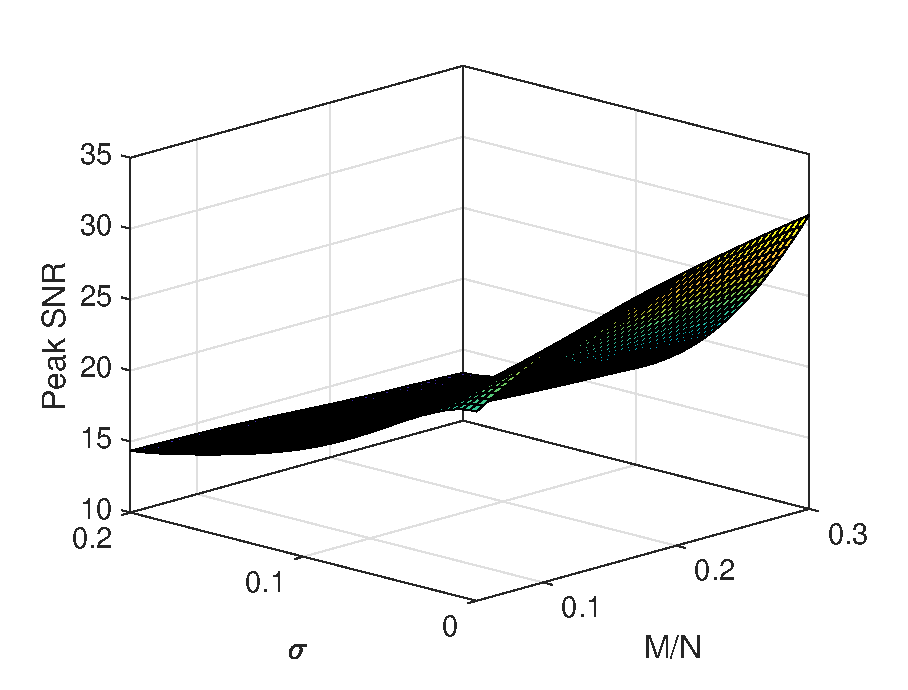
\includegraphics[width = 0.7\linewidth]{result/synt_sss/PSNR_fit.eps}
    \caption{Peak SNR result depending on number of measurements and simulated noise level. $\frac{M}{N}$ is the subsampling ratio and $\sigma$ is the standard deviation added to $\mathbf{y}$.}
    \label{fig:psnr_3d}
\end{figure}

\begin{figure}[H]
    \centering
    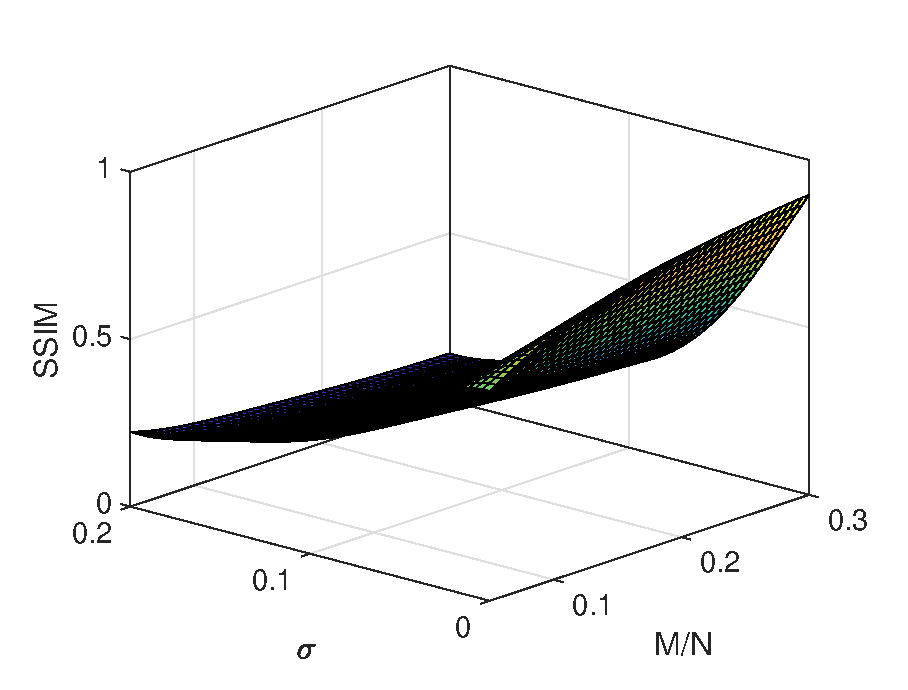
\includegraphics[width = 0.7\linewidth]{result/synt_sss/SSIM_fit.eps}
    \caption{SSIM result depending on number of measurements and simulated noise level. $\frac{M}{N}$ is the subsampling ratio and $\sigma$ is the standard deviation added to $\mathbf{y}$.}
    \label{fig:ssim_3d}
\end{figure}

In both figure~\ref{fig:psnr_3d} and \ref{fig:ssim_3d}, it can be seen that when the noise increases the reconstructed image quality is not improved at the same rate as in the noiseless case, when the subsampling ratio is increased.

\subsection{Reconstruction performance using no reference quality assessment}
In this sub section the same reconstructed image set from section~\ref{sec:reconstruction_performance} is used to calculate the \textit{no reference image quality} with the BRISQUE algorithm.\\[0.1in] 

The results displayed in figure~\ref{fig:Brisque_3d} show that less noise and more samples yield better performance in the reconstruction. The figure also contain the mean results from the "ideal" SWIR images as the flat blue surface, which has scored a far greater score than the reconstructed images.
  

\begin{figure}[H]
    \centering
    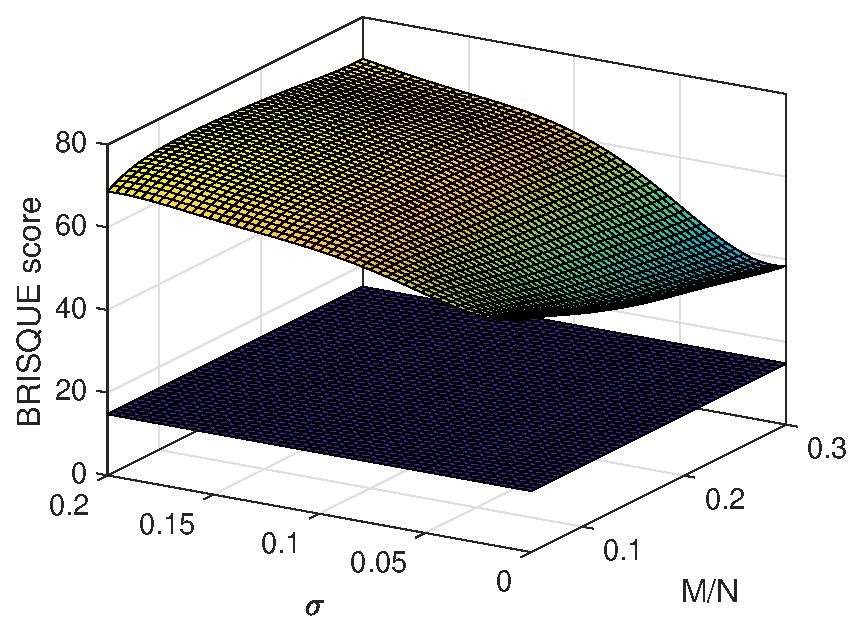
\includegraphics[width = 0.7\linewidth]{result/synt_brisque/BRISQUE_fit.eps}
    \caption{BRISQUE result depending on number of measurements and simulated noise level. Lower surface is reference image score. $\frac{M}{N}$ is the subsampling ratio and $\sigma$ is the standard deviation added to $\mathbf{y}$, lower BRISQUE scores are better.}
    \label{fig:Brisque_3d}
\end{figure}

In figure~\ref{fig:Brisque_2d} the result has been flattened to a 2D graph with fewer selected data points for clarity. In the noiseless case the score will not be better than approximately 40 for the reconstructed images, while the SWIR images have a mean value of 15.


\begin{figure}[H]
    \centering
    \includegraphics[width = 0.95\linewidth]{result/synt_brisque/Brisque_fit_flat3.eps}
    \caption{BRISQUE result depending on number of measurements for different simulated noise levels. $\frac{M}{N}$ is the subsampling ratio and $\sigma$ is the standard deviation added to $\mathbf{y}$, lower BRISQUE scores are better.}
    \label{fig:Brisque_2d}
\end{figure}

In the simulated images with $\sigma > 0.08$ the BRISQUE score start to get unexpected results, first yielding a worse BRISQUE score when increasing the subsampling ratio up to 15-20\%  but then gets better after 20\%, as seen in figure~\ref{fig:Brisque_2d}.
